\begin{figure}[t]
\centering
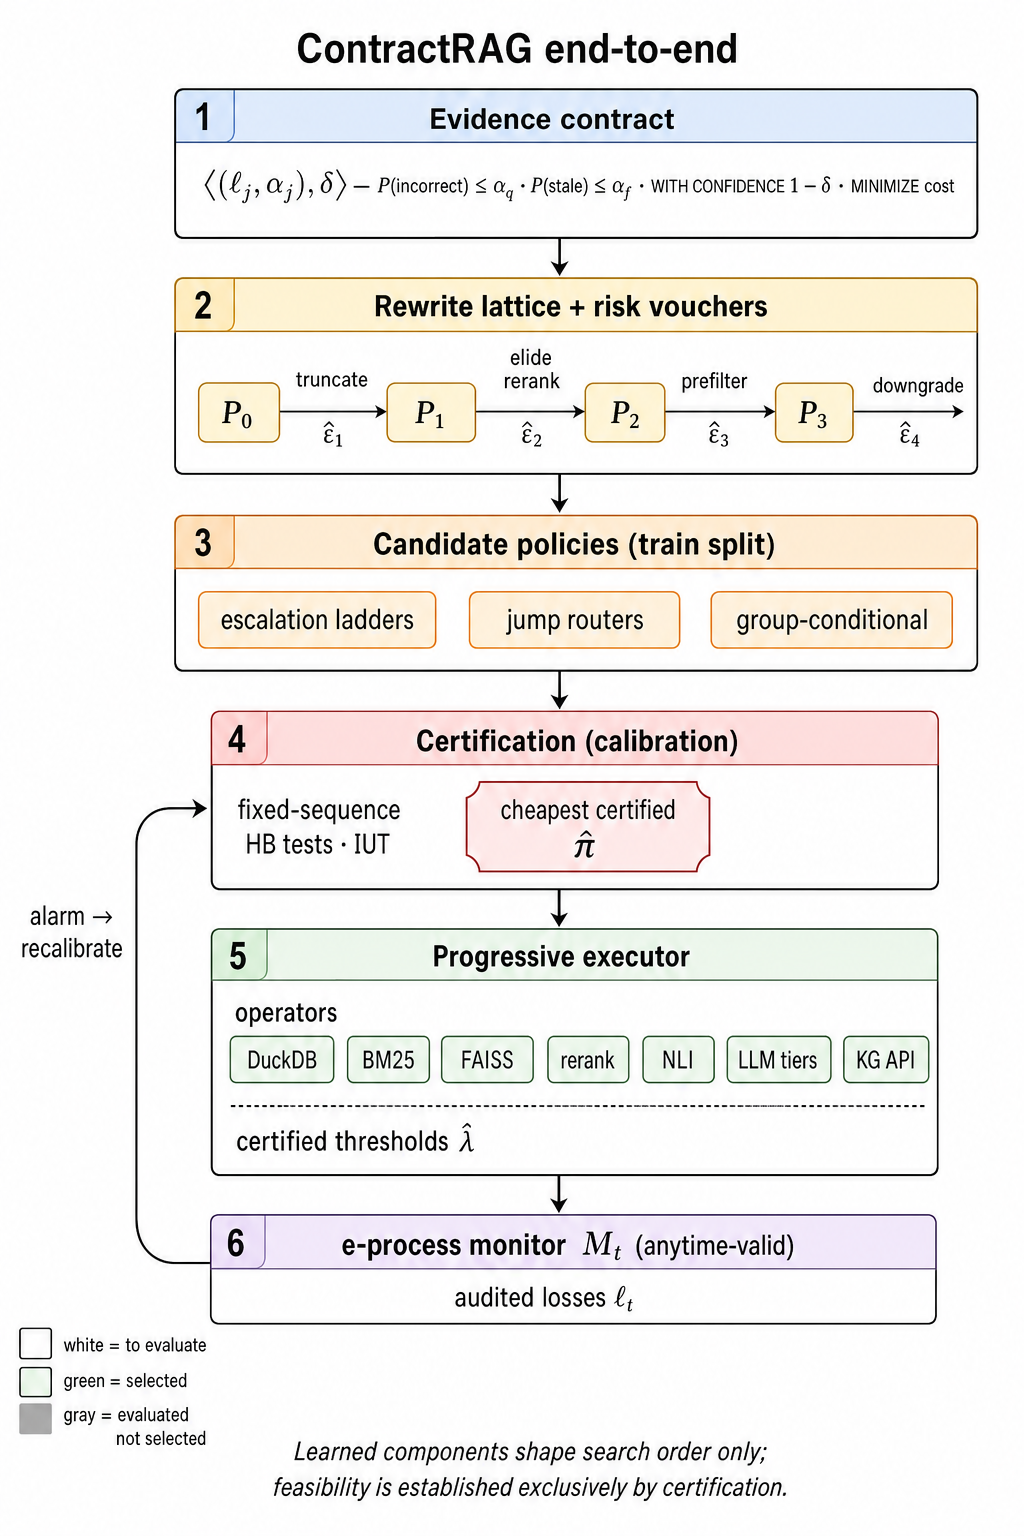
\includegraphics[width=\columnwidth]{figures/fig_arch_imagegen.png}
\caption{\system\ end to end. The application declares a contract (blue);
the rewrite layer generates a voucher-annotated plan lattice and the
policy layer lifts it into adaptive candidates on the train split
(orange); the certification layer walks the candidates with
fixed-sequence tests on the calibration split and deploys the cheapest
certified policy (red); the executor runs it progressively over the
physical operators (green) while the e-process monitor audits realized
losses and triggers recalibration on drift (violet). Learned components
shape only the search order; feasibility is established exclusively by
the red layer.}
\Description{The ContractRAG architecture: evidence contract, rewrite
and policy generation, fixed-sequence certification, progressive
execution, monitoring, and recalibration.}
\label{fig:arch}
\end{figure}
